\begin{figure}[htbp]

\begin{center}
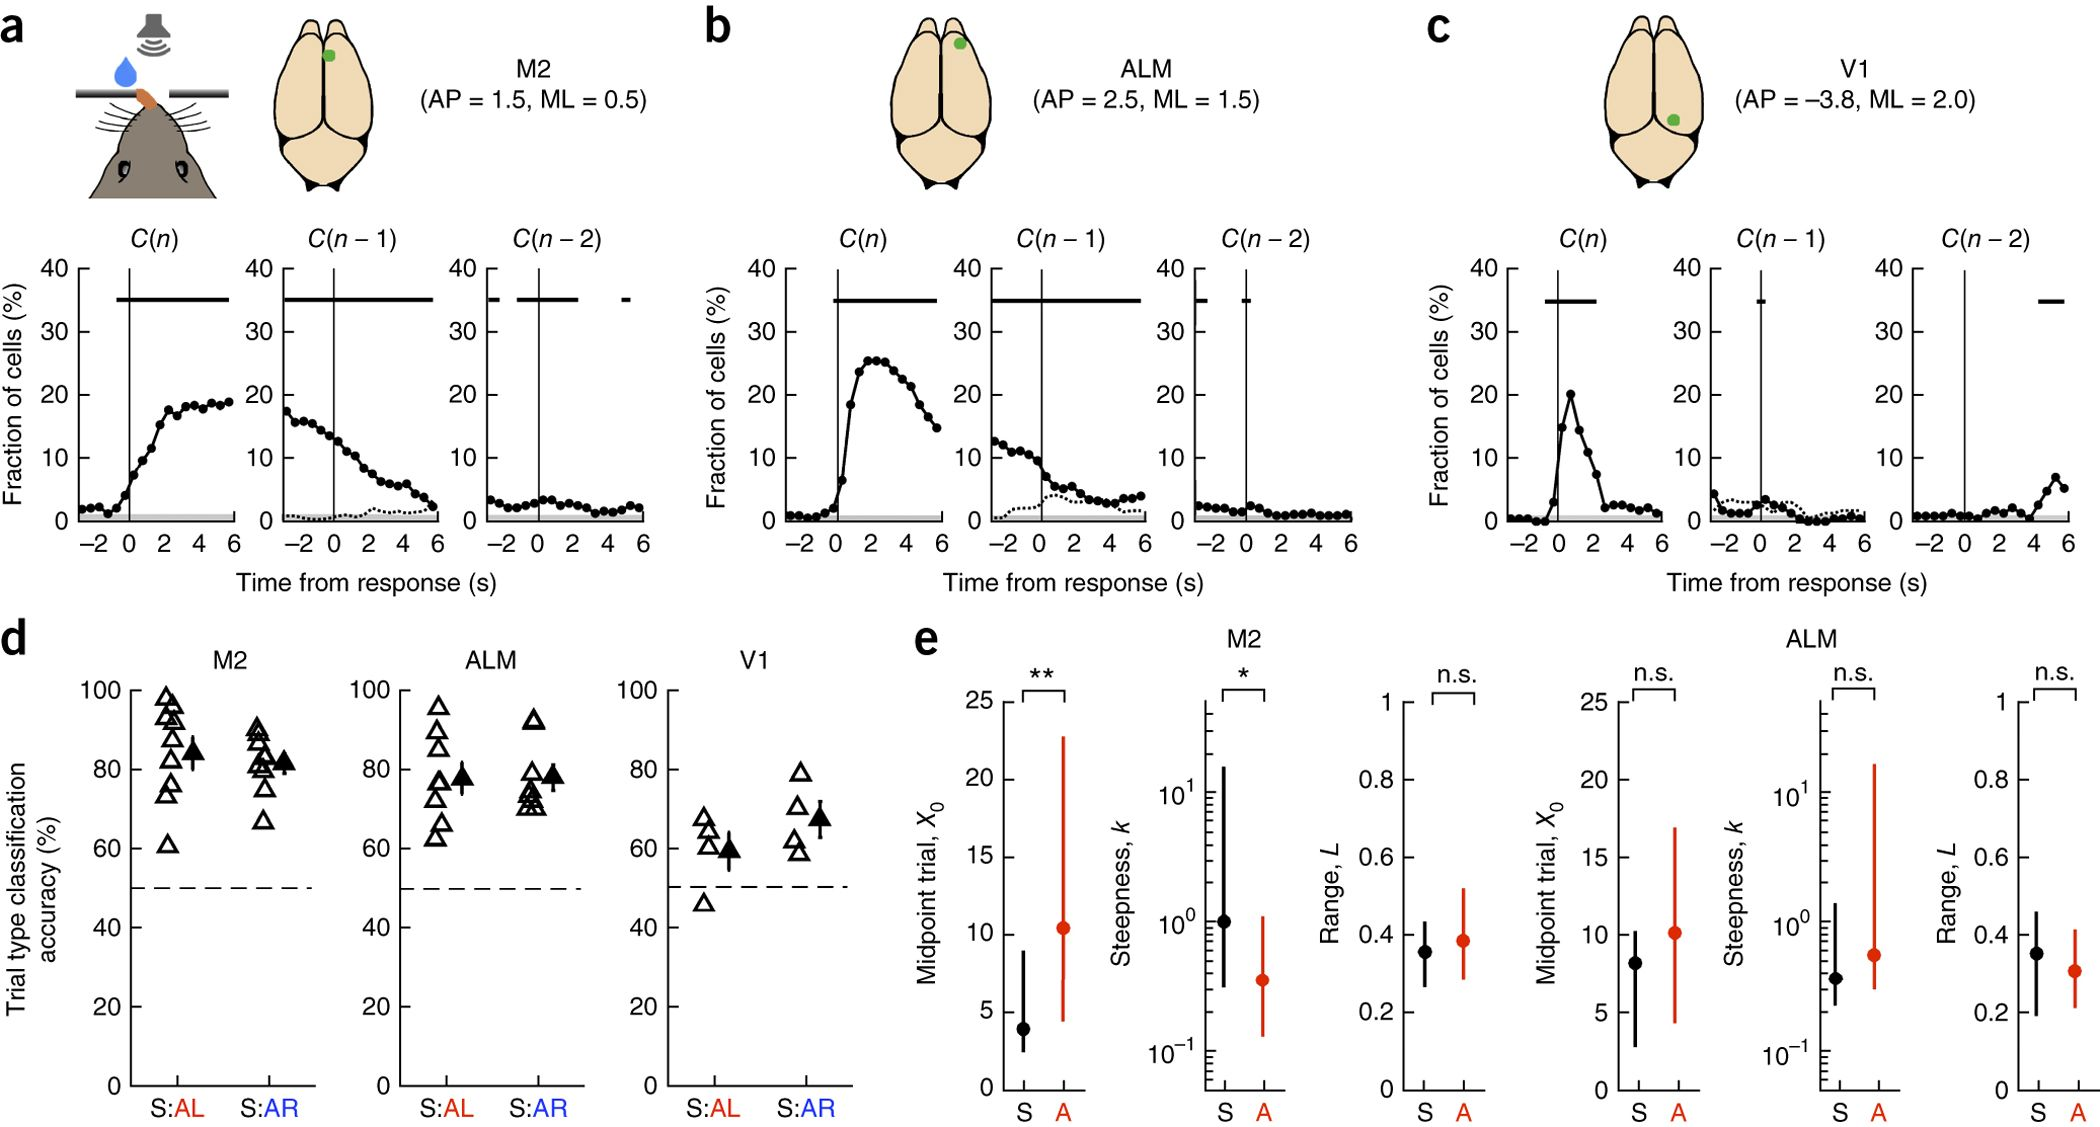
\includegraphics[width=\textwidth]{Figures/Chapter3/NN_fig7} 
\end{center}

\caption[Comparison of neural activity patterns in M2, ALM, and V1]
{
Comparison of neural activity patterns in M2, ALM, and V1 during flexible sensorimotor behavior.
(a) Multiple linear regression analysis was used to evaluate the fraction of 562 M2 neurons encoding choice signals as a function of time. Regression was performed with a moving window ($\mathit{duration} = 0.5$ s, $\mathit{step} = 0.5$ s) to test for significance with $\alpha = 0.01$ on all sound-guided trials where the current and prior choices were rewarded. Black bars, significant fractions ($p < 0.01$, binomial test). Gray shading, significance level of $\alpha=0.01$. Dotted line in the middle panel, fraction of cells significant for the interaction term $C(n) \times C(n-1)$. $N = 9$ sessions from 5 mice. (b) Same as \emph{a} for 518 ALM neurons. $N = 8$ sessions from 4 mice. (c) Same as \emph{a} for 227 V1 neurons. $N = 4$ sessions from 2 mice. (d) Median accuracy of decoding trial type from individual population activity vectors restricted to matched trials, comparing M2, ALM and V1 ensembles. For S:AL, sound or action-left trial types were decoded from trials where the stimulus was an upsweep, choice was left, and outcome was reward for the current trial, and choice was left for the prior trial. For S:AR, sound or action-right trial types were decoded from trials where the stimulus was a downsweep, choice was right, outcome was reward for the current trial, and choice was right for the prior trial. Trial type was decoded with high accuracy using ensemble activity from M2 (matched sound--action-left trials: $84 \pm 4\%$, $t_8 = 8.37$; $p = 3 \times 10^{-5}$; matched sound--action-right trials: $81 \pm 2\%$, $t_8 = 12.73$; $p = 1 \times 10^{-6}$; versus chance level of 50\%, one-sample t-test). Open triangles, individual experiments. Filled triangles, $\mathit{mean}\pm\mathit{SEM}$. Dotted line, chance-level accuracy. (e) Neural transition parameters obtained by fitting action-to-sound (black) and sound-to-action (red) transitions with the logistic function, comparing M2 and ALM ensembles. Wilcoxon rank-sum test, sound vs. action, M2: midpoint trial $x_0$, $p = 0.007$, $z = 2.70$; steepness $k$, $p = 0.03$, $z = -2.17$; height $L$, $p = 0.8$, $z = 0.28$; ALM: $x_0$, $p = 0.11$, $z = 1.62$; $k$, $p = 0.4$, $z = 0.89$; $L$, $p = 0.51$, $z = -0.65$. *$p < 0.05$; **$p < 0.01$; n.s., not significant. Filled circles, medians. Lines end at 25th and 75th percentiles.
}

\label{fig:NN_fig7}
\end{figure}